%%% Preamble
\documentclass[paper=a4, fontsize=11pt]{scrartcl}
\usepackage[spanish, activeacute]{babel} %Definir idioma español
\usepackage[utf8]{inputenc} %Codificacion utf-8
\usepackage{booktabs, multicol, multirow}

\usepackage[T1]{fontenc}
\usepackage{fourier}
\usepackage{multirow}

\usepackage[spanish]{babel}
\usepackage[protrusion=true,expansion=true]{microtype}	
\usepackage{amsmath,amsfonts,amsthm} % Math packages
\usepackage[pdftex]{graphicx}	
\usepackage{url}
\usepackage{listings}
\usepackage[usenames,dvipsnames]{color}
\usepackage{xcolor}
\usepackage{graphicx}
\usepackage{hyperref}

%%% Custom sectioning
\usepackage{sectsty}
\allsectionsfont{\centering \normalfont\scshape}


%%% Custom headers/footers (fancyhdr package)
\usepackage{fancyhdr}
\pagestyle{fancyplain}
\fancyhead{}											% No page header
\fancyfoot[L]{}											% Empty 
\fancyfoot[C]{}											% Empty
\fancyfoot[R]{\thepage}									% Pagenumbering
\renewcommand{\headrulewidth}{0pt}			% Remove header underlines
\renewcommand{\footrulewidth}{0pt}				% Remove footer underlines
\setlength{\headheight}{13.6pt}


%%% Equation and float numbering
\numberwithin{equation}{section}		% Equationnumbering: section.eq#
\numberwithin{figure}{section}			% Figurenumbering: section.fig#
\numberwithin{table}{section}				% Tablenumbering: section.tab#


%%% Maketitle metadata
\newcommand{\horrule}[1]{\rule{\linewidth}{#1}} 	% Horizontal rule

\lstset{ %
  backgroundcolor=\color{white},   % choose the background color; you must add \usepackage{color} or \usepackage{xcolor}
  basicstyle=\footnotesize,        % the size of the fonts that are used for the code
  breakatwhitespace=false,         % sets if automatic breaks should only happen at whitespace
  breaklines=true,                 % sets automatic line breaking
  captionpos=b,                    % sets the caption-position to bottom
  commentstyle=\color{red},    % comment style
  deletekeywords={...},            % if you want to delete keywords from the given language
  escapeinside={\%*}{*)},          % if you want to add LaTeX within your code
  extendedchars=true,              % lets you use non-ASCII characters; for 8-bits encodings only, does not work with UTF-8
  frame=single,                    % adds a frame around the code
  keepspaces=true,                 % keeps spaces in text, useful for keeping indentation of code (possibly needs columns=flexible)
  keywordstyle=\color{orange},       % keyword style
  language=Python,                 % the language of the code
  morekeywords={*,...},            % if you want to add more keywords to the set
  numbers=left,                    % where to put the line-numbers; possible values are (none, left, right)
  numbersep=5pt,                   % how far the line-numbers are from the code
  numberstyle=\tiny\color{gray}, % the style that is used for the line-numbers
  rulecolor=\color{black},         % if not set, the frame-color may be changed on line-breaks within not-black text (e.g. comments (green here))
  showspaces=false,                % show spaces everywhere adding particular underscores; it overrides 'showstringspaces'
  showstringspaces=false,          % underline spaces within strings only
  showtabs=false,                  % show tabs within strings adding particular underscores
  stepnumber=0,                    % the step between two line-numbers. If it's 1, each line will be numbered
  stringstyle=\color{green},     % string literal style
  tabsize=2,                       % sets default tabsize to 2 spaces
  %title=\lstname                   % show the filename of files included with \lstinputlisting; also try caption instead of title
}

\title{
		%\vspace{-1in} 	
		\usefont{OT1}{bch}{b}{n}
		\normalfont \normalsize \textsc{UNIVERSIDAD TÉCNICA FEDERICO SANTA MARÍA\\
CAMPUS SANTIAGO\\
DEPARTAMENTO DE INFORMÁTICA\\
REDES DE COMPUTADORES
} \\ [25pt]
		\horrule{0.5pt} \\[0.4cm]
		\huge Informe Tarea 3 \\
		\horrule{2pt} \\[0.5cm]
}


\author{
\normalfont 
  Ignacio Sfeir\\[-3pt]
  \normalfont \normalsize
  ignacio.sfeir@alumnos.usm.cl\\[-3pt]
  \normalfont \normalsize
  201104725-7\\[-3pt]
  \and
  \normalfont 
  Mat\'ias Ramirez\\[-3pt]
  \normalfont \normalsize
  matias.ramirezm@alumnos.usm.cl\\[-3pt]
  \normalfont \normalsize
  201173506-4\\[-3pt]
  \and \normalfont
  \today
}

\date{}


%%% Begin document
\begin{document}
\maketitle


\clearpage \newpage

\section*{Open Visual Traceroute}

\subsection*{Pregunta 1}
\paragraph{} \hspace{0pt}

Existen una serie de cables submarinos intercontinentales de fibra \'optica, los cuales permiten el traspaso de informaci\'on (paquetes) entre los distintos continentes. La siguiente imagen muestra el recorrido de estos cables a trav\'es del mundo:\\

\graphicspath{{fotos/}}

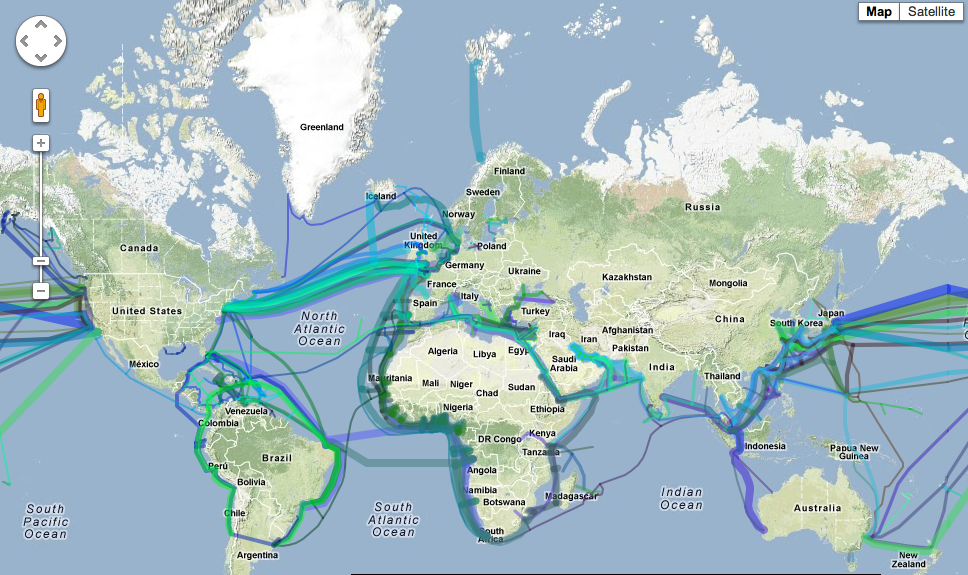
\includegraphics[width=1\textwidth]{under-sea-cable-map.png}

Naturalmente surge  la pregunta; ¿Porque cables en vez de señales satelitales? La respuesta es confiabilidad, velocidad y latencia. en caso de que un cable falle por alg\'un motivo, los dem\'as pueden asumir la carga hasta que sea arreglado. Adem\'as los cables de fibra \'optica tienen una mayor velocidad de transferencia, y generan una menor cantidad de latencia que las señales satelitales, aunque su gran inconveniente es que cuestan cientos de millones de dólares construirlos.\\

Chile cuenta con tres de estos cables:\\
\begin{enumerate}
\item Panamericano (PanAm), que llega por el Oceano Pac\'ifico hasta Arica.\\
\item South America-1 (SAm-1), llega hasta Arica y Valpara\'iso.\\
\item South American Crossing (SAC)/Latin American Nautilus (LAN), que llega desde el Pac\'ifico hasta Valpara\'iso.\\
\end{enumerate}

A continuación se muestran los pantallazos para verificar que se realizó el traceroute:\\

Moodle:\\\\
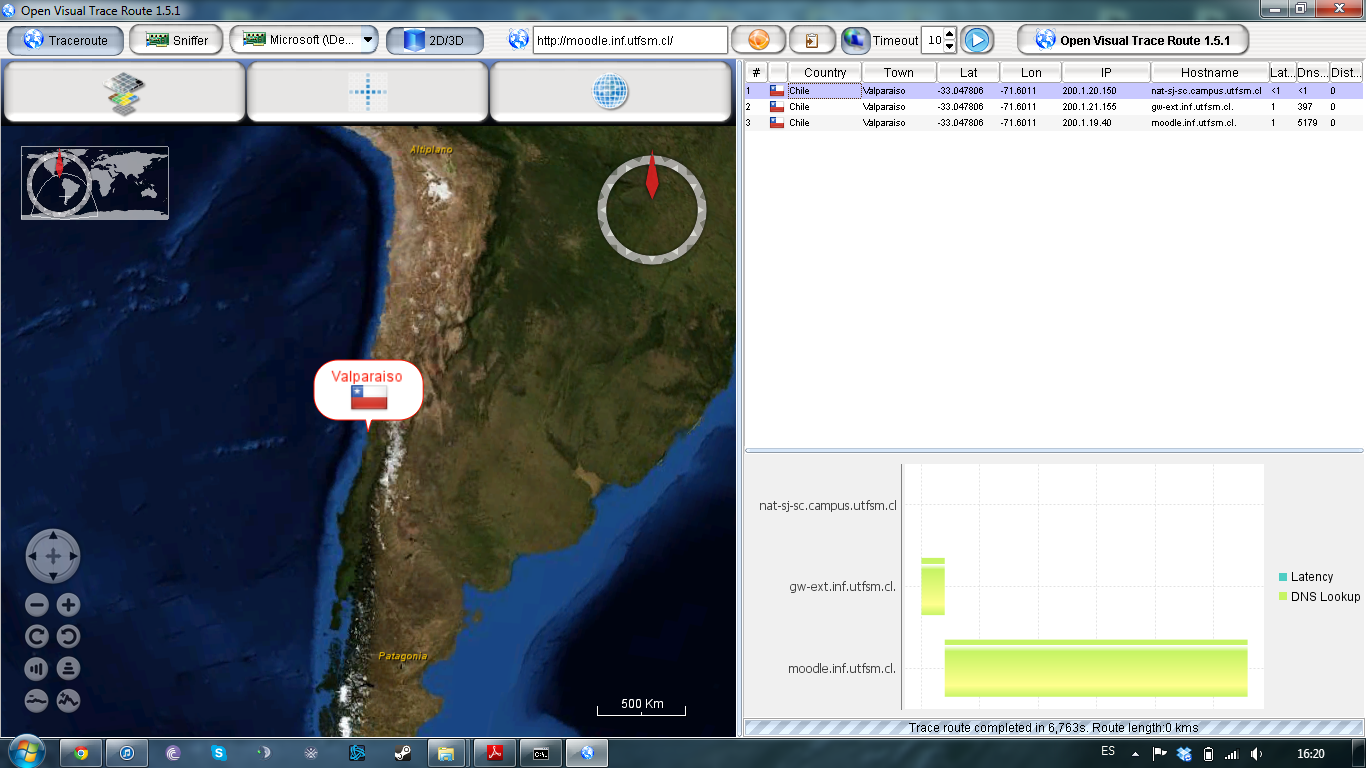
\includegraphics[width=1\textwidth]{moodle.png}\\\\
Cime:\\\\
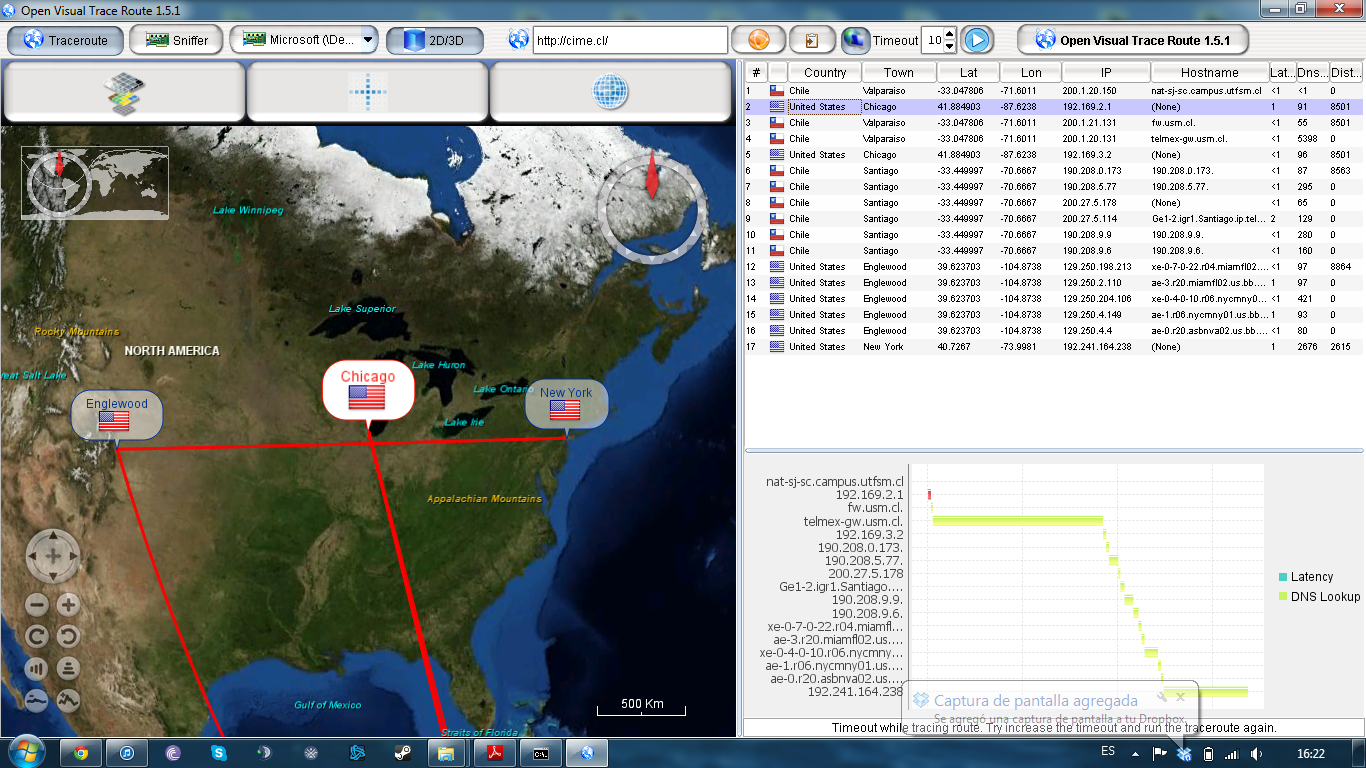
\includegraphics[width=1\textwidth]{cime.png}
\clearpage
Google:\\\\
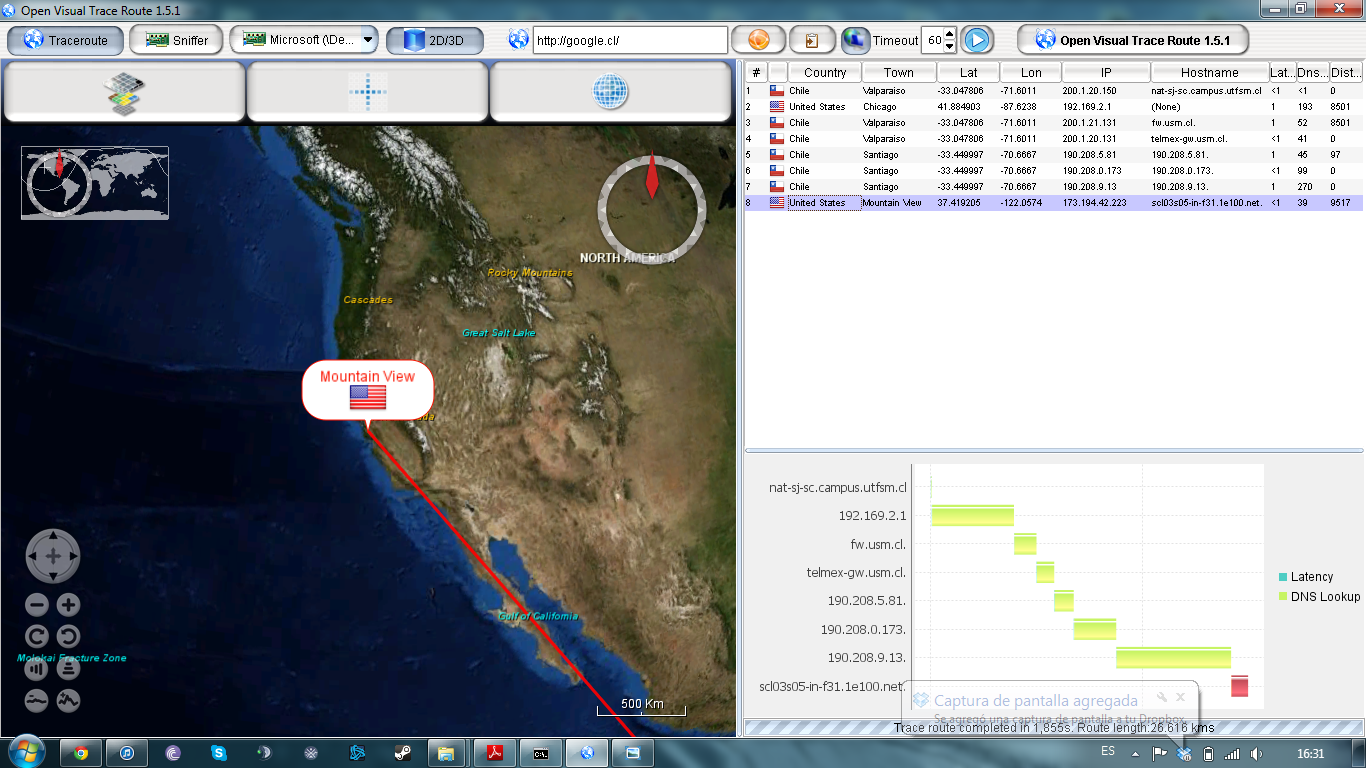
\includegraphics[width=1\textwidth]{google.png}\\\\
Wikipedia:\\\\
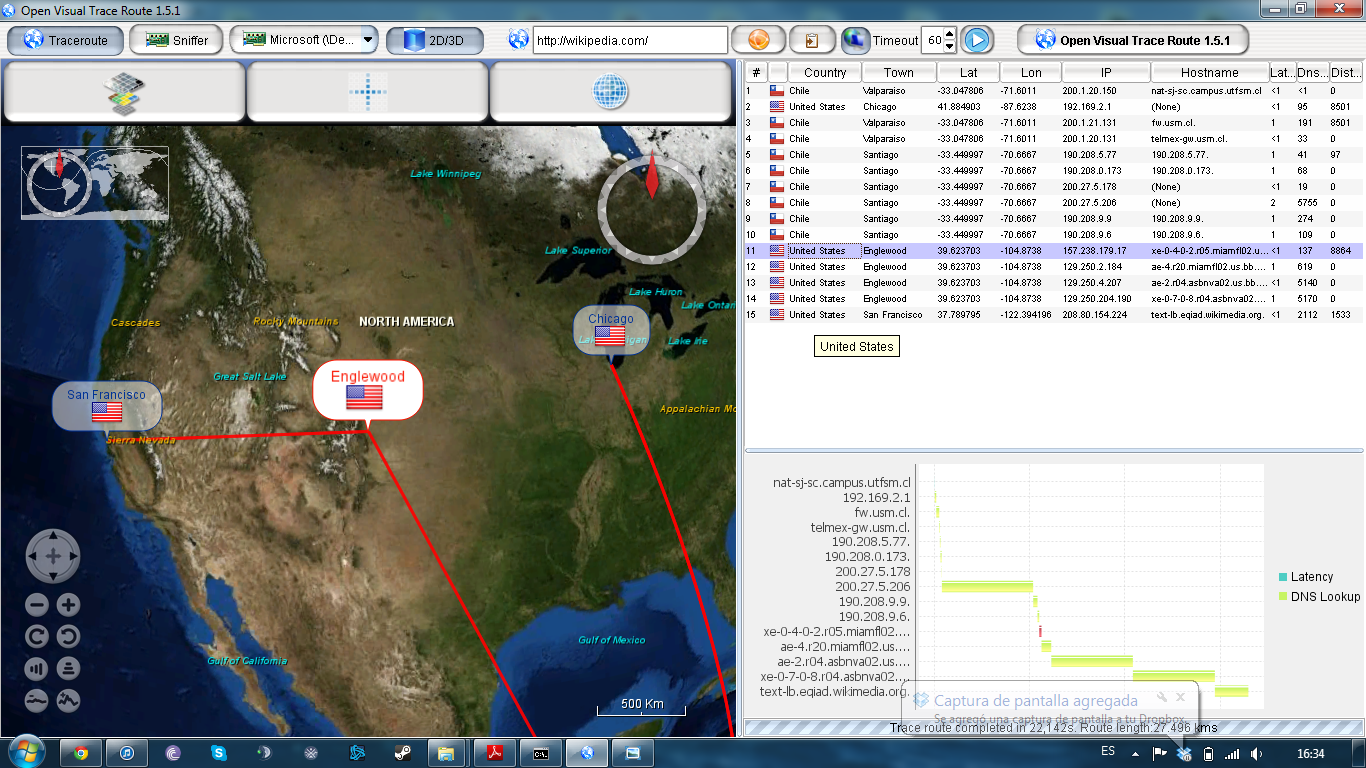
\includegraphics[width=1\textwidth]{wikipedia.png}
\clearpage
Embassy:\\\\
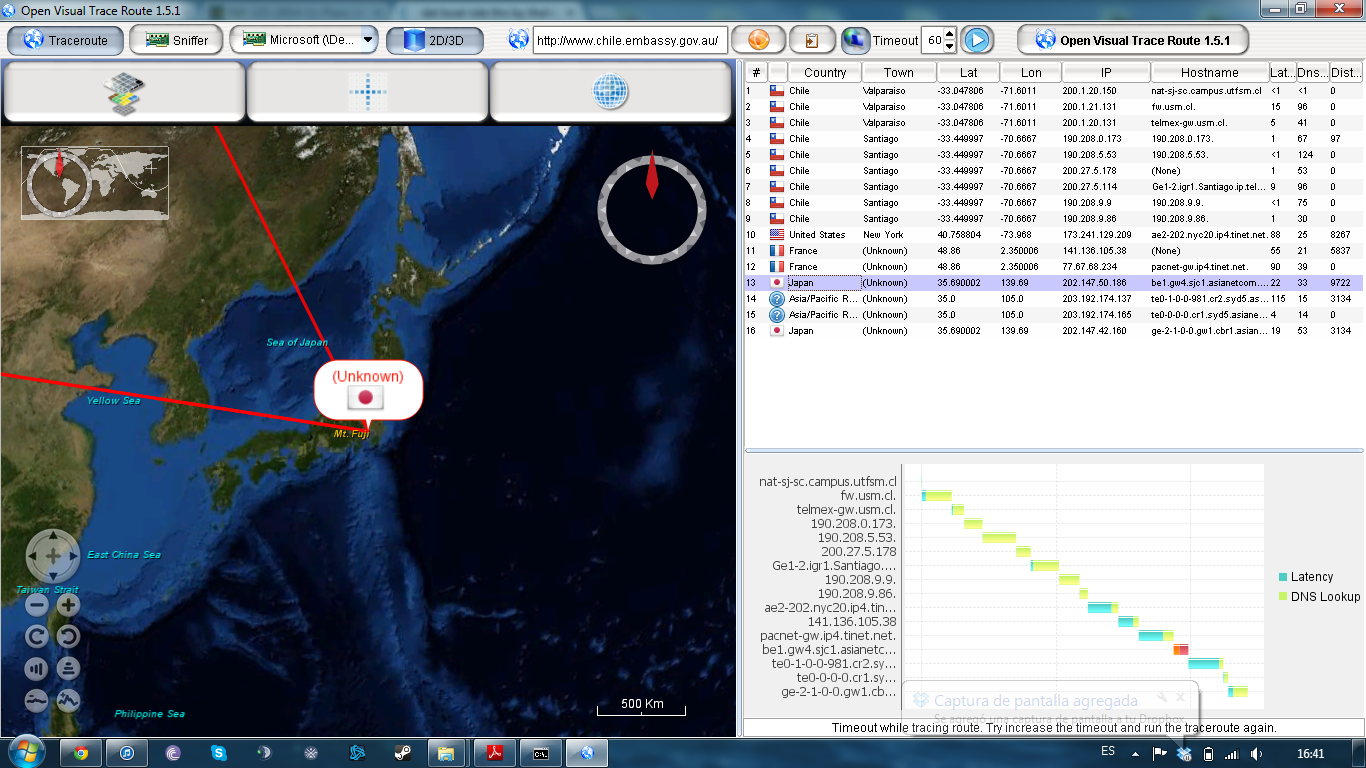
\includegraphics[width=1\textwidth]{embassy.png}\\\\

La ruta que toman los paquetes, mostrada en Open Visual Traceroute, es determinada por varios factores. Uno de ellos es el uso de proxy web, el cual recibe la URL de pedida y la busca en su caché local, de estar ahí la envía de inmediato de vuelta al usuario, y en caso contrario realiza una petición a otro servidor, el cual puede ser el principal, u otro proxy. La petición que realiza el servidor proxy es compartida por múltiples usuarios, por lo tanto hay una mejora en los tiempos de acceso para consultas coincidentes y además se libera carga a los enlaces de acceso a Internet, al disminuir la cantidad de peticiones realizadas.
Cabe destacar que existen métodos para elegir el camino ''menos congestionado'' a través de algoritmos de enrutamiento.

\clearpage

\section*{Algoritmo Vector-Distancia}

\subsection*{Pregunta 2}
\paragraph{} \hspace{0pt}

A continuación se mostrará el proceso completo paso por paso del algoritmo vector distancia para los routers del grafo entregado:\\

\graphicspath{{tablas/}}

Nodo A
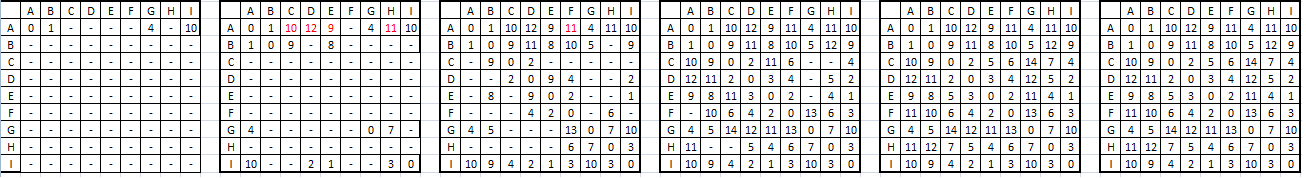
\includegraphics[width=1\textwidth]{2a.png}\\\\
Nodo B
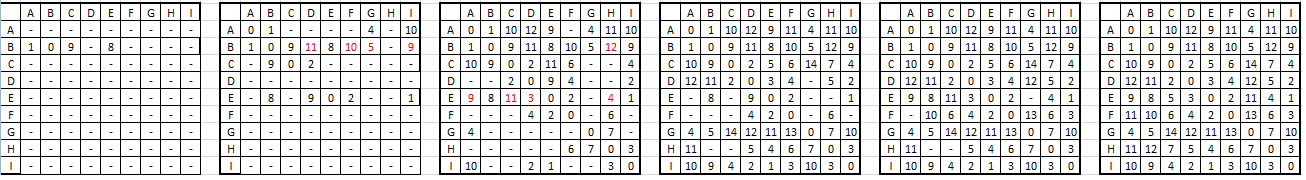
\includegraphics[width=1\textwidth]{2b.png}\\\\
Nodo C
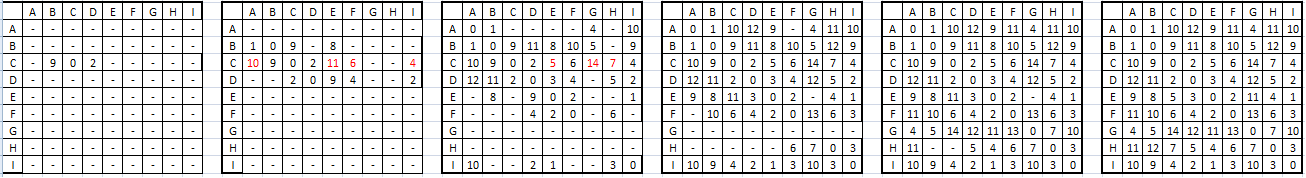
\includegraphics[width=1\textwidth]{2c.png}\\\\
Nodo D
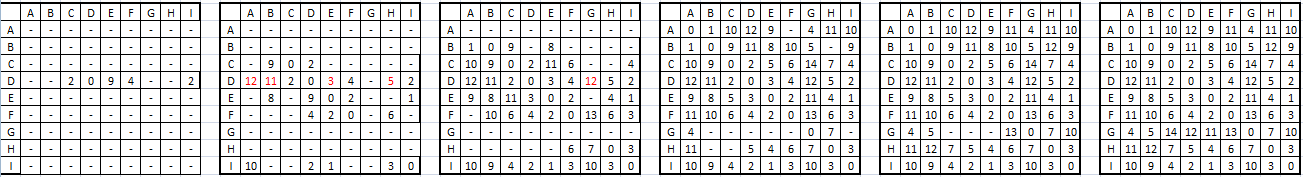
\includegraphics[width=1\textwidth]{2d.png}\\\\
Nodo E
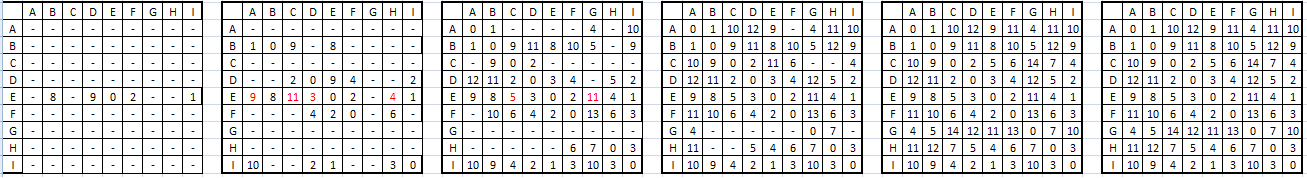
\includegraphics[width=1\textwidth]{2e.png}\\\\
Nodo F
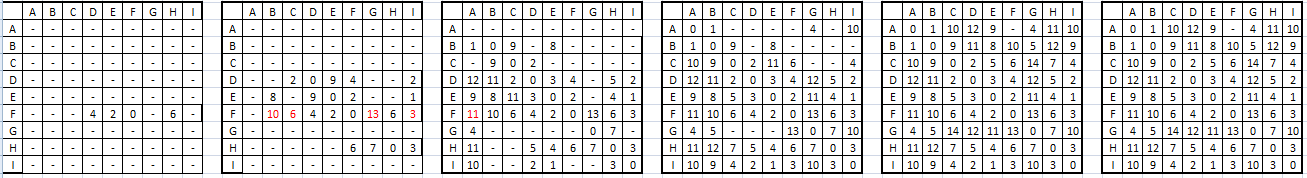
\includegraphics[width=1\textwidth]{2f.png}\\\\
Nodo G
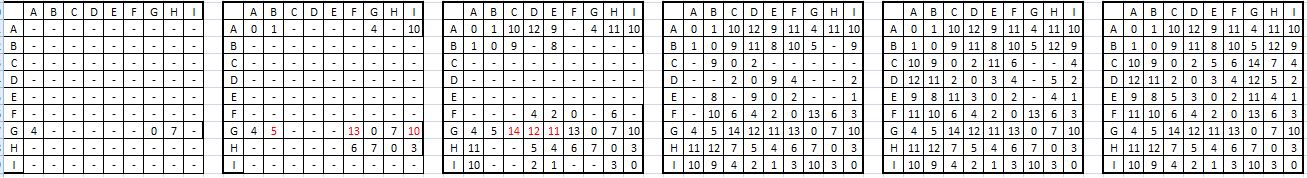
\includegraphics[width=1\textwidth]{2g.png}\\\\
Nodo H
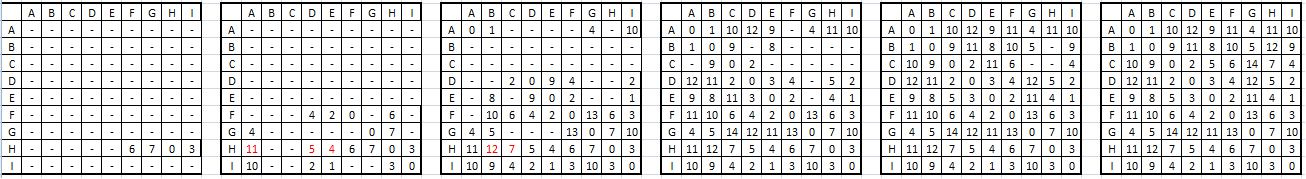
\includegraphics[width=1\textwidth]{2h.png}\\\\
Nodo I
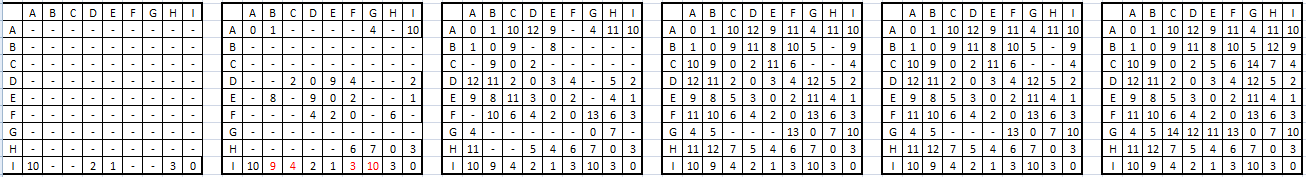
\includegraphics[width=1\textwidth]{2i.png}\\\\




\subsection*{Pregunta 3}
\paragraph{} \hspace{0pt}

Ahora con el enlace entre H e I roto, esos dos nodos comienzan a informar a sus vecinos de esto y se procede a reparar la matriz de costos del grafo.\\

Nodo A
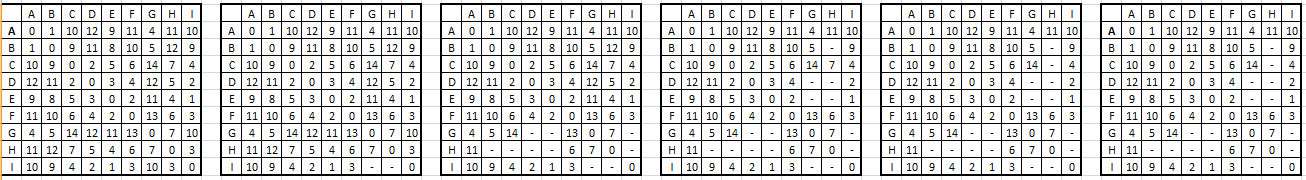
\includegraphics[width=1\textwidth]{3a1.png}\\
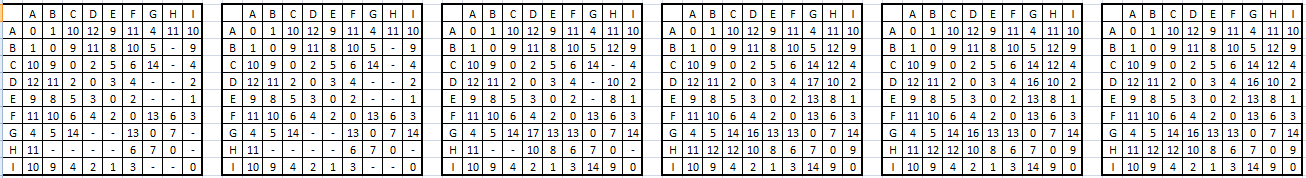
\includegraphics[width=1\textwidth]{3a2.png}\\\\
Nodo B
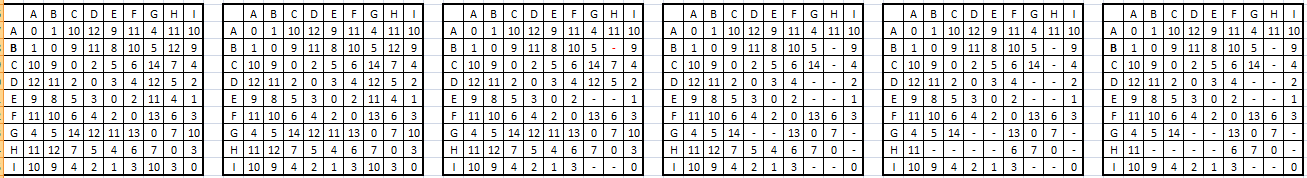
\includegraphics[width=1\textwidth]{3b1.png}\\
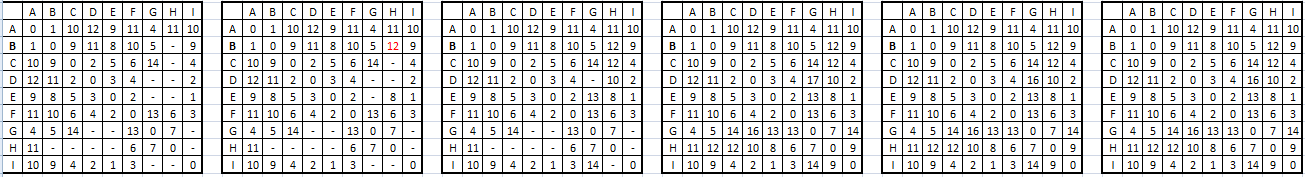
\includegraphics[width=1\textwidth]{3b2.png}\\\\
Nodo C
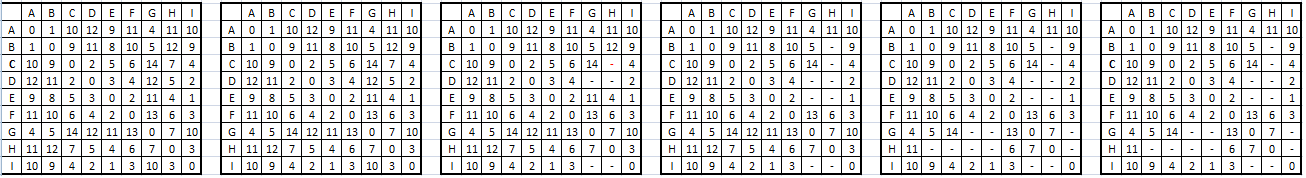
\includegraphics[width=1\textwidth]{3c1.png}\\
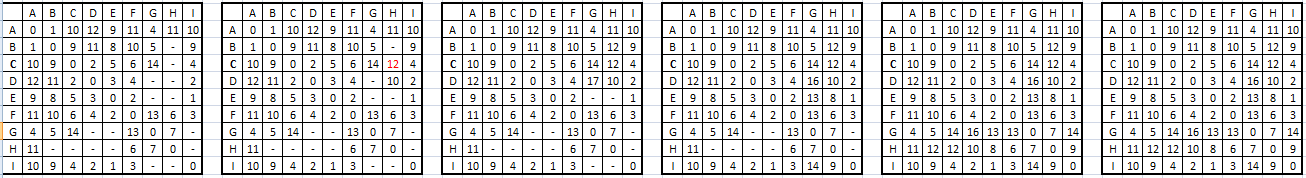
\includegraphics[width=1\textwidth]{3c2.png}\\\\
Nodo D
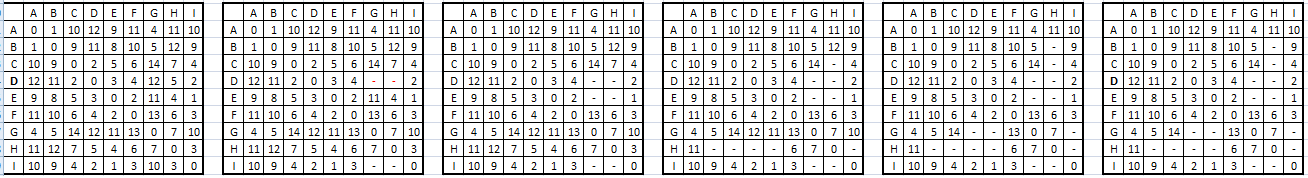
\includegraphics[width=1\textwidth]{3d1.png}\\
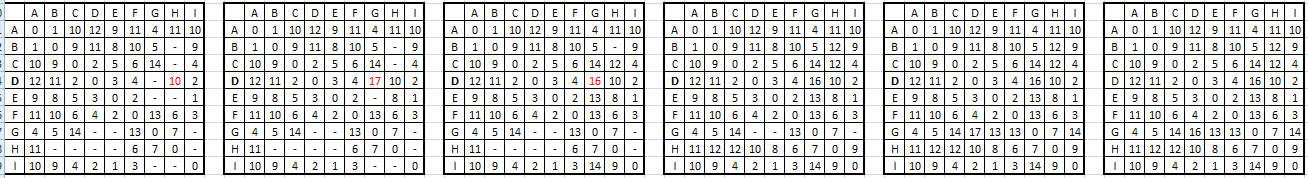
\includegraphics[width=1\textwidth]{3d2.png}\\\\
Nodo E
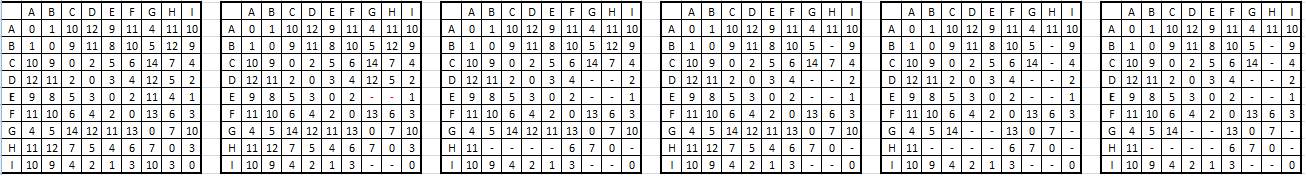
\includegraphics[width=1\textwidth]{3e1.png}\\
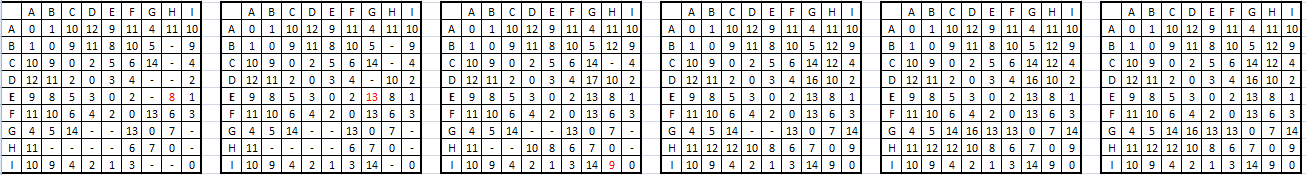
\includegraphics[width=1\textwidth]{3e2.png}\\\\
Nodo F
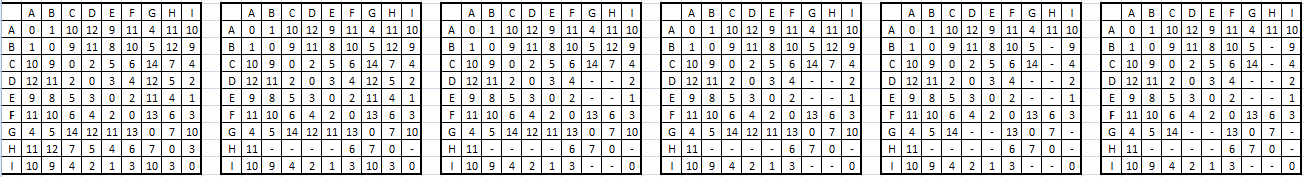
\includegraphics[width=1\textwidth]{3f1.png}\\
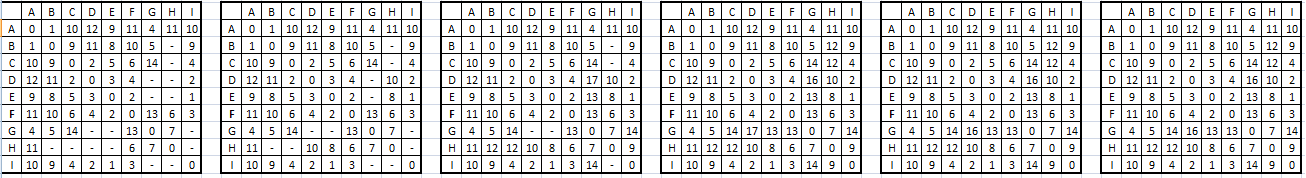
\includegraphics[width=1\textwidth]{3f2.png}\\\\
Nodo G
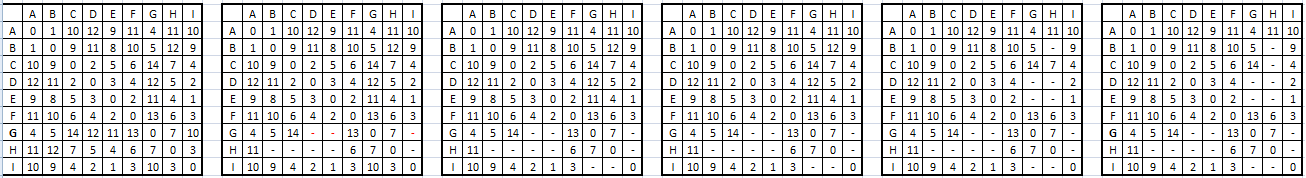
\includegraphics[width=1\textwidth]{3g1.png}\\
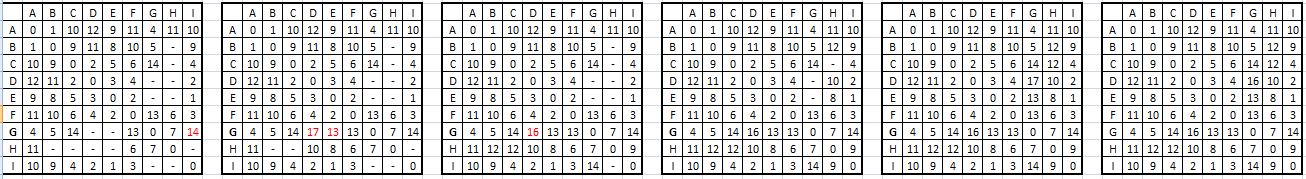
\includegraphics[width=1\textwidth]{3g2.png}\\\\
Nodo H
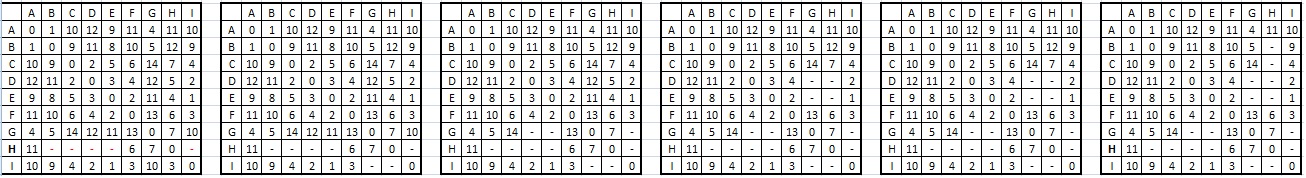
\includegraphics[width=1\textwidth]{3h1.png}\\
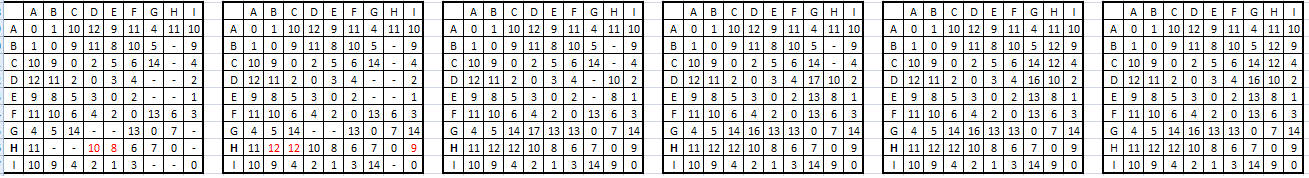
\includegraphics[width=1\textwidth]{3h2.png}\\\\
Nodo I
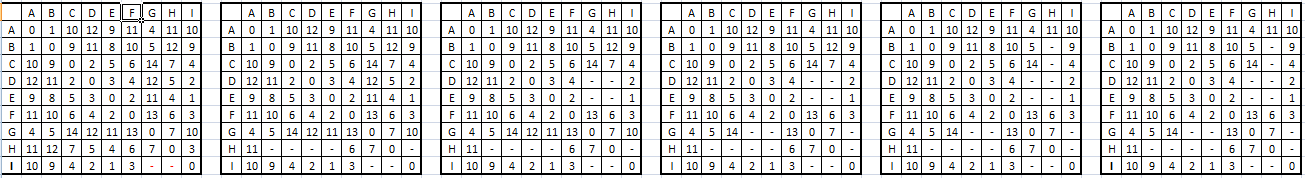
\includegraphics[width=1\textwidth]{3i1.png}\\
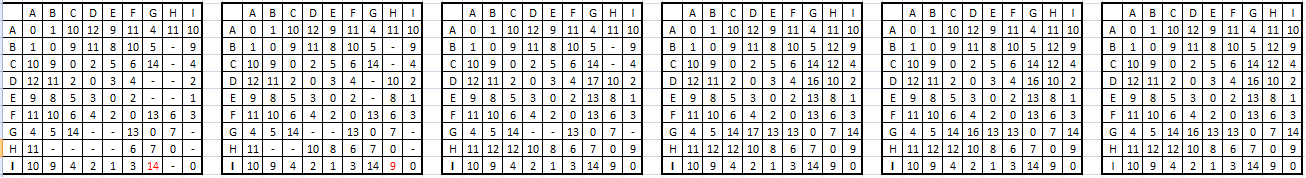
\includegraphics[width=1\textwidth]{3i2.png}\\\\


\end{document}